% !TEX root = handbook-physics.tex
% !TEX TS-program = pdflatex
% !TEX encoding = UTF-8 Unicode




\chapter{Fundamentals Of Quantum Optics}
\label{ch-37}
\zhtitle{量子光学基础}

\section[External Photoelectric Effect]{External Photoelectric Effect
(Photoemissive Effect)}
\label{sec-37.1} 
\zhtitle{外光电效应（光电发射效应）}

\subsection{}\label{37.1.1} \redem{Quantum optics} is the branch of optics that studies phenomena in which the quantum properties of light are manifested. Such phenomena include thermal radiation \ssect{36.1.1}, the photoelectric effect, the Compton effect \ssect{37.3.1} and photochemical processes.
\zhpar{\redem{量子光学}是光学的一个分支，研究光的量子性质所表现出来的各种现象。这类现象包括热辐射\ssect{36.1.1}、光电效应、康普顿效应\ssect{37.3.1}以及光化学过程等。}

The \redem{photoelectric effect} in gases consists in the ionization of the atoms and molecules of the gas due to the action of light, and is usually called \redem{photoionization}.
\zhpar{气体中的\redem{光电效应}是指光的作用使气体的原子和分子发生电离，通常称为\redem{光电离}。}

In condensed bodies (liquids and solids) distinction is made
between the external and internal photoelectric effects.
\zhpar{在凝聚态物质（液体和固体）中，通常区分外光电效应和内光电效应。}

The \redem{external photoelectric effect (photoemission)} is the emission of electrons by a substance subject to the action of light. Electrons ejected from the substance in the external photoelectric effect are called photoelectrons, and the electric current formed by them in their ordered motion in the external electric field is called the photoelectric current.
\zhpar{\redem{外光电效应（光电发射）}是指物质在光的作用下发射电子的现象。外光电效应中从物质中逸出的电子称为光电子，光电子在外电场中定向运动所形成的电流称为光电流。}

The \redem{internal photoelectric effect} is the redistribution of electrons among the energy states in solid and liquid semiconductors and dielectrics due to the action of light. It is manifested in the change in the concentration of current carriers in a medium \ssect{20.1.4} and leads to photoconduction or the barrier-layer photoelectric
effect. 
\zhpar{\redem{内光电效应}是指光的作用使固体和液体半导体及电介质中的电子在各能态之间重新分布的现象。它表现为介质中载流子浓度的变化\ssect{20.1.4}，并导致光电导或阻挡层光电效应。}
\begin{marginfigure}[-1cm] 
\centering
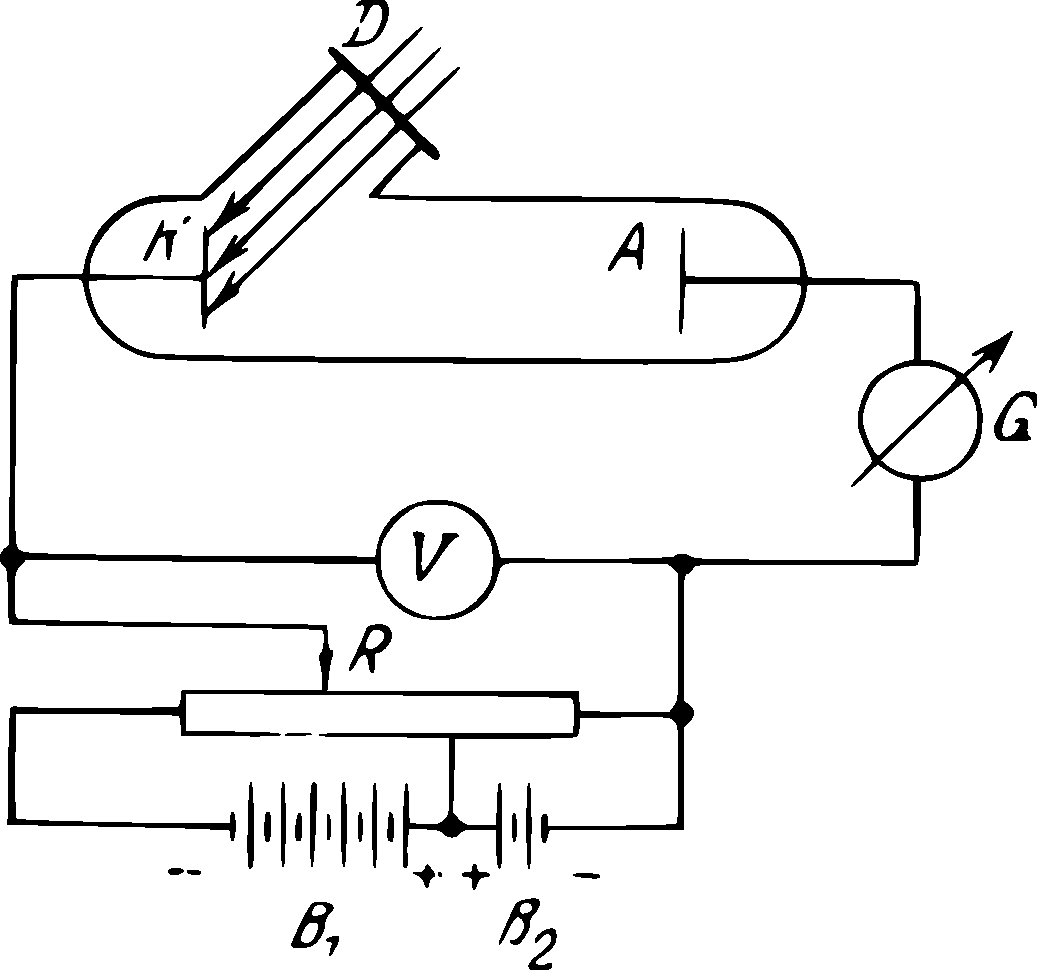
\includegraphics[width=\textwidth]{figs/ch-37/fig-37-01.pdf}
\sidecaption{Investigating the external photoelectric effect in metals.\zhcap{研究金属中外光电效应的装置。}\label{fig-37-01}}
\end{marginfigure}

\redem{Photoconduction} is an increase in the electrical
conductivity of a substance due to light falling on it. The \redem{barrier-layer photoelectric effect} is the generating of an emf (photo-emf) by the action of light in a system consisting of a semiconductor and metal in contact or two different kinds of semiconductors [for example at a \emph{p-n} junction \ssect{41.11.7}].
\zhpar{\redem{光电导}是指物质受光照射时电导率增大的现象。\redem{阻挡层光电效应}是指光的作用在由半导体与金属相接触，或由两种不同类型的半导体组成的体系中产生电动势（光电动势）的现象[例如在\emph{p-n}结\ssect{41.11.7}处]。}

\begin{marginfigure}[3cm] 
\centering
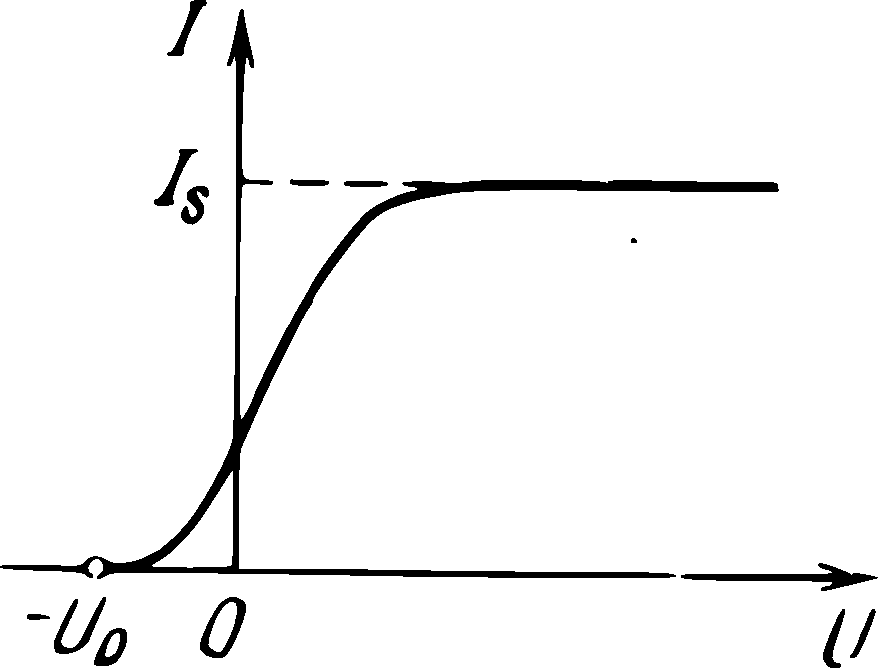
\includegraphics[width=\textwidth]{figs/ch-37/fig-37-02.pdf}
\sidecaption{The dependene of photoelectric current on potential difference in the tube.\zhcap{光电流随管中电势差的变化关系。}\label{fig-37-02}}
\end{marginfigure}


\subsection{}\label{37.1.2} Shown in \figr{fig-37-01} is an installation for investigating the external photoelectric effect in metals. Light enters through window $D$ and falls on the surface of cathode $K$, which is inside a vacuum tube and is called the \redem{photoelectric cathode}. The shape of the curve, representing the dependence of the photoelectric
current $I$ in the tube on the potential difference $U$ between the anode $A$ and cathode $K$ upon constant irradiance $E_{e}$ of the cathode \ssect{36.4.2} by monochromatic light, is shown in \figr{fig-37-02}.
\zhpar{如\figr{fig-37-01}所示为研究金属中外光电效应的装置。光从窗口$D$射入，照射到位于真空管内的阴极$K$表面上，该阴极称为\redem{光电阴极}。在阴极辐照度$E_{e}$\ssect{36.4.2}保持不变、以单色光照射的条件下，管中光电流$I$随阳极$A$与阴极$K$之间电势差$U$的变化曲线如\figr{fig-37-02}所示。}


The existence of a photoelectric current at negative values of $U$ from 0 to $- U_{0}$ indicates that the photoelectrons have a certain initial velocity when emitted from the cathode, and the corresponding kinetic energy. The maximum initial velocity $v_{max}$ of the photoelectrons is related to the \redem{retarding voltage (retarding potential)} $U_{0}$ by the equation 
\zhpar{当$U$在$0$到$-U_{0}$的负值范围内时仍存在光电流，表明光电子从阴极逸出时具有一定的初速度及相应的动能。光电子的最大初速度$v_{max}$与\redem{遏止电压（遏止电势）}$U_{0}$之间的关系由下式给出：}
\begin{equation*}%
\frac{mv^{2}_{max}}{2} = eU_{0},
\end{equation*}
where $e$ and $m$ are the absolute values of the charge and the mass of the electron.
\zhpar{式中$e$和$m$分别为电子电荷和电子质量的绝对值。}

The photoelectric current increases with $U$ only to a definite
limiting value $I_{S}$ called the \redem{saturation photoelectric current}. At this value, all the electrons escaping from the cathode, due to the effect of light, reach the anode. If $n_{sec}$ is the number of photoelectrons emitted from the cathode per second, then
\zhpar{光电流随$U$的增大只能增加到某一确定的极限值$I_{S}$，该值称为\redem{饱和光电流}。在此值下，光照下从阴极逸出的全部电子都到达阳极。若$n_{sec}$为每秒从阴极发射的光电子数，则有}
\begin{equation*}%
I_{S} = en_{sec}.
\end{equation*}

\subsection{}\label{37.1.3} The external photoelectric effect obeys the following laws.
\zhpar{外光电效应服从下列规律。}
\begin{enumerate}[label=\arabic*.]
\item The \redem{Stoletov law} slates that at a constant spectral composition of the light incident upon the photoelectric cathode, the saturation photoelectric current is proportional to the irradiance \ssect{36.4.2} of the cathode:
\zhpar{\redem{斯托列托夫定律}指出：当射到光电阴极上的光的光谱成分保持不变时，饱和光电流与阴极的辐照度\ssect{36.4.2}成正比：}
\begin{equation*}%
I_{S} \propto E_{e} \qand n_{sec} \propto E_{e}.
\end{equation*}
\item For a given photoelectric cathode, the initial velocity of the photoelectrons depends upon the frequency of the light, but not on its intensity.
\zhpar{对于给定的光电阴极，光电子的初速度取决于光的频率，而与光的强度无关。}
\item A \redem{photoelectric threshold} exists for each photoelectric cathode, i.e. the minimum frequency $\nu_{0}$ of light at which the external photoelectric effect is still feasible. This frequency $\nu_{0}$ depends upon the material of the photoelectric cathode and the condition of its surface.
\zhpar{每一种光电阴极都存在\redem{光电效应红限}，即能够产生外光电效应的最低光频率$\nu_{0}$。该频率$\nu_{0}$取决于阴极材料及其表面状况。}
\end{enumerate}
The second and third laws cannot be interpreted on the basis
of the classical electromagnetic theory of light. According to
this theory the removal of conduction electrons from the metal
is a result of their ``swaying'' in the electromagnetic field of the light wave so that they are ``loosened''. This effect should increase with the light intensity and with the irradiance of the photoelectric cathode, proportional to the intensity.
\zhpar{第二、第三条规律无法用光的经典电磁理论解释。按照该理论，金属中传导电子的逸出是由于光波的电磁场使电子“摆动”从而被“松脱”。这种效应应随光强以及与光强成正比的光电阴极辐照度的增大而增强。}

\subsection{}\label{37.1.4} Only the quantum theory of light enabled the laws of the external photoelectric effect to be properly explained. In a further development of Planck's ideas on the quantization of the energy of atoms (oscillators) \ssect{36.3.2}, Einstein proposed the hypothesis that light is not only radiated, but also propagates in space and is absorbed by matter in the form of separate discrete quanta of electromagnetic radiation, which were named \redem{photons}. All photons of monochromatic light of the frequency v have the same energy $E_{ph}= h\nu$, where $h$ is Planck's constant, and travel in space at the velocity $c$ of light in vacuum (or in free space). In the absorption of light each absorbed photon transmits all of its energy to a particle of the absorbing substance.
\zhpar{只有光的量子理论才能正确解释外光电效应的规律。在普朗克关于原子（振子）能量量子化思想\ssect{36.3.2}的进一步发展中，爱因斯坦提出假设：光不仅在辐射时是量子化的，而且在空间中传播以及被物质吸收时，也是以分立的电磁辐射量子形式存在的，这些量子被称为\redem{光子}。频率为$\nu$的单色光的所有光子都具有相同的能量$E_{ph}= h\nu$，其中$h$为普朗克常量，它们以真空中（或自由空间中）的光速$c$传播。光被吸收时，每个被吸收的光子将其全部能量传递给吸收物质的一个粒子。}

In the external photoelectric effect, for example, a conduction
electron of the metal, in absorbing a photon, receives
all of its energy $h\nu$. The work function $\Phi$ \ssect{41.11.1} is the minimum energy that it is necessary to impart to the electron for it to escape from a metal. Hence, \redem{Einstein's photoelectric emission equation}, expressing the law of the conservation of energy in the photoelectric effect, is of the form
\zhpar{例如，在外光电效应中，金属中的一个传导电子吸收一个光子时获得其全部能量$h\nu$。\redem{逸出功}$\Phi$\ssect{41.11.1}是使电子从金属中逸出所必须传给电子的最小能量。因此，表示光电效应中能量守恒定律的\redem{爱因斯坦光电效应方程}具有如下形式：}
\begin{equation*}%
h \nu = \Phi + \frac{mv^{2}_{max}}{2}.
\end{equation*}

\subsection{}\label{37.1.5} The second law of the photoelectric effect follows directly from Einstein's equation:
\zhpar{由爱因斯坦方程可直接得出光电效应的第二条规律：}
\begin{equation*}%
\frac{mv^{2}_{max}}{2} = eU_{0} = h \nu - \Phi. 
\end{equation*}
Thus, $v_{max}$ and $U_{0}$ depend only upon the frequency of the light and the work function in emitting an electron from the photoelectric cathode.
\zhpar{因此，$v_{max}$和$U_{0}$仅取决于光的频率以及从光电阴极中发射电子所需的逸出功。}

The maximum initial kinetic energy of the photoelectrons depends upon the light frequency according to a linear relation. It becomes zero at the frequency $\nu_{0}$, corresponding to the photoelectric threshold. Thus
\zhpar{光电子的最大初动能随光频率按线性关系变化。在频率$\nu_{0}$处它变为零，该频率对应于光电效应红限。于是有}
\begin{equation*}%
\nu_{0} = \frac{\Phi}{h}.
\end{equation*}
Consequently, the photoelectric threshold depends only on the
electron work function of the metal.
\zhpar{因此，光电效应红限仅取决于金属的电子逸出功。}

\subsection{}\label{37.1.6} The photoelectric effect is inertialess, i.e. the emission of photoelectrons begins immediately, as soon as light with the frequency $\nu \geqslant \nu_{0}$ falls on the photoelectric cathode. This feature of the external photoelectric effect is still another confirmation of the quantum nature of interaction between light and matter. According to classical wave conceptions, quite considerable time is required for an electromagnetic wave of given intensity to impart sufficient energy to the electron for its emission from the metal.
\zhpar{光电效应无惯性，即只要频率$\nu \geqslant \nu_{0}$的光一照射到光电阴极上，光电子的发射就立即开始。外光电效应的这一特征进一步证明了光与物质相互作用的量子本质。按照经典波动概念，具有一定强度的电磁波需要相当长的时间才能把足够的能量传给电子，使其从金属中逸出。}

\subsection{}\label{37.1.7} At very high intensities of light, achieved by means of lasers \ssect{39.8.8}, a \redem{multiple-photon}, or \redem{nonlinear photoelectric effect} is observed. In this case, the electron can simultaneously receive the energy of $N$ photons rather than that of one photon. Then the equation of the law of conservation of energy in the external photoelectric effect under the action of light of frequency
$\nu$ is of the form
\zhpar{当光强非常高时（借助激光器\ssect{39.8.8}获得），会观察到\redem{多光子光电效应}，又称\redem{非线性光电效应}。在这种情况下，电子可以同时吸收$N$个光子的能量，而不是一个光子的能量。于是，在频率为$\nu$的光作用下，外光电效应中能量守恒定律的方程为}
\begin{equation*}%
N h \nu = \Phi + \frac{mv^{2}_{max}}{2}.
\end{equation*}
The photoelectric threshold of the $N$-photon photoelectric effect is
\zhpar{$N$光子光电效应的红限为：}
\begin{equation*}%
(\nu_{0})_{N} = \frac{\Phi}{Nh}.
\end{equation*}


\section{Mass and Momentum of the Photon. Light Pressure}
\label{sec-37.2} 
\zhtitle{光子的质量和动量。光压}


\subsection{}\label{37.2.1} The \redem{mass of the photon} \ssect{37.1.4} having the energy $E_{ph}= h\nu$, where $\nu$ is the frequency of the light and $h$ is Planck's constant, can be found from the mass-energy relation \ssect{5.7.2}.
Thus
\zhpar{光子的能量为$E_{ph}= h\nu$\ssect{37.1.4}，其中$\nu$为光的频率，$h$为普朗克常量。光子的质量可由质能关系\ssect{5.7.2}求得。于是有}
\begin{equation*}%
m_{ph} = \frac{h \nu}{c^{2}}.
\end{equation*}
where $c$ is the velocity of light in free space (or in a vacuum). The photon always travels with the velocity $c$, and its rest mass \ssect{5.6.1}  equals zero.
\zhpar{式中$c$为自由空间（或真空）中的光速。光子总是以速度$c$运动，其静止质量\ssect{5.6.1}为零。}

\subsection{}\label{37.2.2} The \redem{momentum $\vb{p}_{ph}$ of the photon} is numerically equal to 
\zhpar{光子的\redem{动量$\vb{p}_{ph}$}的数值等于}
\begin{equation*}%
p_{ph} = m_{ph} c = \frac{h \nu}{c} = \frac{h}{\lambda}.
\end{equation*}
where $\lambda$ is the wavelength of the light in vacuum. Since the wavenumber is $k = 2\pi/\lambda$,
\zhpar{式中$\lambda$为真空中光的波长。由于波数为$k = 2\pi/\lambda$，故有}
\begin{equation*}%
p_{ph} = \frac{h}{2 \pi} k = \hbar k \qand \vb{p}_{ph} = \hbar \vb{k},
\end{equation*}
where $\hbar = h/2\pi$, and $\vb{k}$ is the wave vector \ssect{30.2.7}.
\zhpar{式中$\hbar = h/2\pi$，$\vb{k}$为波矢\ssect{30.2.7}。}


\begin{marginfigure}%[-3cm] 
\centering
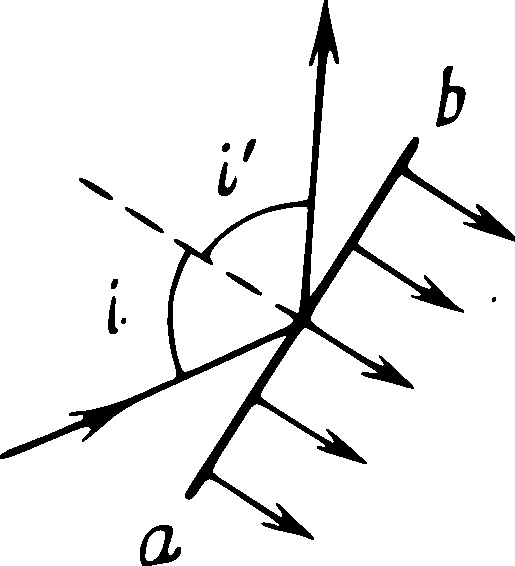
\includegraphics[width=0.75\textwidth]{figs/ch-37/fig-37-03.pdf}
\sidecaption{Analysing pressure of light falling on a surface of a body.\zhcap{分析照射到物体表面上的光压。}\label{fig-37-03}}
\end{marginfigure}

\subsection{}\label{37.2.3} Light exerts a pressure on the bodies that reflect or absorb it. In quantum optics, light pressure is interpreted as the result of the transfer of momentum to bodies by photons as the light is reflected or
absorbed. The \redem{light pressure} $p$ on the plane
surface $ab$ of a body (\figr{fig-37-03}) is equal to the numerical value of the normal component of the total momentum transferred by photons to the body on unit area of the surface being considered during unit time.
\zhpar{光照射到能够反射或吸收光的物体上会产生压力。在量子光学中，光压被解释为光被反射或吸收时光子把动量传递给物体的结果。物体平面表面$ab$上的\redem{光压}$p$（见\figr{fig-37-03}）等于单位时间内、单位面积上光子传递给物体的总动量在表面法线方向上的分量的数值。}

Assume that monochromatic light of frequency $\nu$ is incident upon surface $ab$ at the angle $i$ (\figr{fig-37-03}) and that $n_{sec}$ is the number of photons incident per second upon unit area of surface $ab$. If $R$ is the coefficient of reflection \ssect{31.5.6} of light from the surface being considered, then, of the $n_{sec}$ photons, $R\, n_{sec}$
are reflected and $(1 - R) n_{sec}$ are absorbed. The photons being reflected transfer a total momentum to the body, directed normal to the surface ab and numerically equal to
\zhpar{设频率为$\nu$的单色光以入射角$i$射到表面$ab$上（见\figr{fig-37-03}），$n_{sec}$为每秒射到表面$ab$单位面积上的光子数。若$R$为所考虑表面对光的反射系数\ssect{31.5.6}，则在$n_{sec}$个光子中，$R\, n_{sec}$个被反射，$(1 - R) n_{sec}$个被吸收。被反射的光子传递给物体的总动量垂直于表面$ab$，其数值等于}
\begin{equation*}%
R \, n_{sec} \frac{2 h \nu}{c} \cos i.
\end{equation*}
The photons being absorbed transfer a total momentum to the
body, whose component normal to surface $ab$ is numerically
equal to
\zhpar{被吸收的光子传递给物体的总动量，其垂直于表面$ab$的分量数值等于}
\begin{equation*}%
(1 - R) \, n_{sec} \frac{ h \nu}{c} \cos i.
\end{equation*}
Thus the light pressure equals
\zhpar{因此，光压等于}
\begin{align*}%
p & = R \, n_{sec} \frac{2 h \nu}{c} \cos i + (1 - R) \, n_{sec} \frac{ h \nu}{c} \cos i \\
& = (1 + R) n_{sec} \frac{ h \nu}{c} \cos i .
\end{align*}
If $n_{0}$ is the photon concentration of the incident light, then $n_{sec} = n_{0} c \cos i$ and $n_{0} h \nu = \expval{E^{d}}$ is the average value of the volume energy density of the light. Hence
\zhpar{若$n_{0}$为入射光的光子浓度，则$n_{sec} = n_{0} c \cos i$，且$n_{0} h \nu = \expval{E^{d}}$为光的体积能量密度的平均值。于是有}
\begin{equation*}%
p = n_{0} h \nu (1 + R) \cos^{2} i = \expval{E^{d}}(1 + R) \cos^{2} i.
\end{equation*}
Thus, the pressure of light can be equally well explained by
either wave theory \ssect{31.2.6} or quantum theory.
\zhpar{因此，光压既可以用波动理论\ssect{31.2.6}解释，也可以同样好地用量子理论解释。}

\section{Compton Effect}
\label{sec-37.3}
\zhtitle{康普顿效应}

\subsection{}\label{37.3.1} The \redem{Compton effect} is the change in the wavelength of $X$-rays when they are scattered by a substance containing lightweight atoms. The wavelength $\lambda'$ of the radiation, scattered at the angle $\theta$ to the direction of propagation of the primary monochromatic
radiation of wavelength $\lambda$, is longer than $\lambda'$, by the amount $\Delta \lambda$, which depends only on angle $\theta$. Thus
\zhpar{\redem{康普顿效应}是指$X$射线被含有轻原子的物质散射时波长发生改变的现象。以与波长为$\lambda$的入射单色辐射传播方向成角$\theta$散射的辐射，其波长$\lambda'$比$\lambda$长，增加量为$\Delta \lambda$，且$\Delta \lambda$只取决于角$\theta$。于是有}
\begin{equation*}%
\Delta \lambda = \lambda' - \lambda  = 2 \lambda_{C} \sin^{2} \frac{\theta}{2}.
\end{equation*}
The constant $\lambda_{C}  = \SI{2.43d-12}{\meter}$ is called the \redem{Compton wavelength of the electron}. The Compton effect cannot be explained on the basis of the classical wave theory of light.
\zhpar{常量$\lambda_{C}  = \SI{2.43d-12}{\meter}$称为\redem{电子康普顿波长}。康普顿效应无法用经典光波理论解释。}

\subsection{}\label{37.3.2} According to quantum theory, the Compton effect is the result of elastic collision of the $X$-ray photon with a free or effectively free electron (in light atoms, the binding energy of an electron with the atom is substantially less than the energy of an $X$-ray photon). In this collision the photon transfers part of its energy and a part of its momentum to the electron in accordance with the laws of the conservation of energy and momentum. If the electron was initially at rest, it follows from the law mv
of conservation of energy that
\zhpar{按照量子理论，康普顿效应是$X$射线光子与自由电子或实际上可视为自由的电子发生弹性碰撞的结果（在轻原子中，电子与原子的结合能远小于$X$射线光子的能量）。在这一碰撞中，光子依照能量守恒和动量守恒定律，将其部分能量和部分动量传递给电子。若电子起始时静止，则由能量守恒定律可得}
\begin{equation*}%
h\nu + m_{0}c^{2} = h\nu' + mc^{2}, \tag{a}
\end{equation*}
where $\nu = c/ \lambda$ and $\nu' = c/ \lambda'$ are the
frequencies of the incident and scattered radiation, $m_{0}c^{2}$ is the rest energy of the electron \ssect{5.7.3}, and $mc^{2}$ is the total energy of the electron \ssect{5.7.2} after the collision (energy of the \redem{Compton recoil electron}).
\zhpar{其中$\nu = c/ \lambda$和$\nu' = c/ \lambda'$分别为入射和散射辐射的频率，$m_{0}c^{2}$为电子的静止能量\ssect{5.7.3}，$mc^{2}$为碰撞后电子的总能量\ssect{5.7.2}（即\redem{康普顿反冲电子}的能量）。}

\begin{marginfigure}%[-3cm] 
\centering
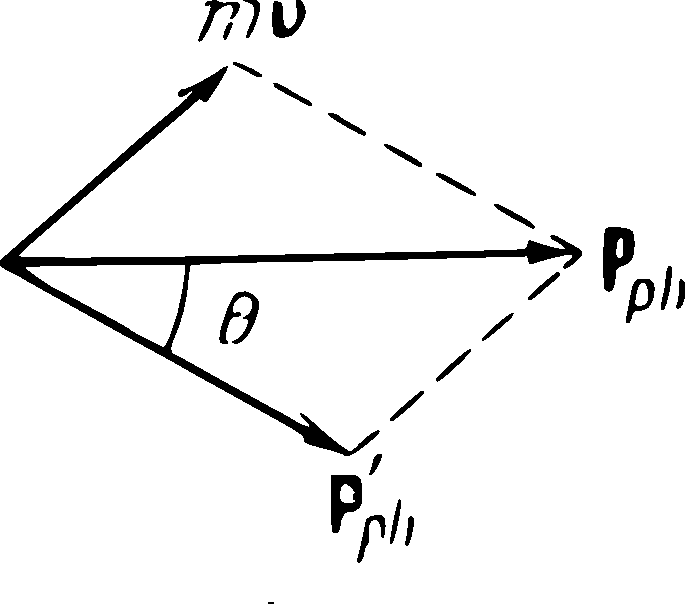
\includegraphics[width=0.8\textwidth]{figs/ch-37/fig-37-04.pdf}
\sidecaption{Investigating Compton scattering.\zhcap{研究康普顿散射的装置。}\label{fig-37-04}}
\end{marginfigure}


It follows from the law of conservation of momentum that
\zhpar{由动量守恒定律可得}
\begin{equation*}%
\vb{p}_{ph} = m\vb{v} + \vb{p}'_{ph},
\end{equation*}
or, in accordance with \figr{fig-37-04},
\zhpar{或按\figr{fig-37-04}所示的关系，}
\begin{equation*}%
(mv)^{2}\left(\frac{h \nu}{c} \right)^{2} +\left(\frac{h \nu'}{c} \right)^{2} - 2 \frac{h^{2}\nu \nu'}{c^{2}} \cos \theta,
\tag{b}
\end{equation*}
where $v$ is the velocity of the Compton recoil electron.
\zhpar{式中$v$为康普顿反冲电子的速度。}

The mass of the recoil electron is related to its velocity $v$ by the equation \ssect{5.6.1}
\zhpar{反冲电子的质量与其速度$v$之间的关系由下式给出\ssect{5.6.1}：}
\begin{equation*}%
m = \frac{m_{0}}{\sqrt{1 - (v/c)^{2}}}. \tag{c}
\end{equation*}
Combining equations (a), (b) and (c), we obtain
\zhpar{联立式(a)、(b)和(c)，可得}
\begin{align*}%
m_{0}c^{2}(\nu - \nu') & = 2 h \nu \nu' \sin^{2} \frac{\theta}{2} \qor \\
\Delta \lambda & = \lambda' - \lambda = \frac{2h}{m_{0}c} \sin^{2} \frac{\theta}{2}.
\end{align*}
Thus, the \redem{Compton wavelength of the electron} is
\zhpar{因此，\redem{电子康普顿波长}为}
\begin{equation*}%
\lambda_{C} = \frac{h}{m_{0}c}.
\end{equation*}


\subsection{}\label{37.3.3} The kinetic energy of the recoil electron \ssect{5.7.1} is
\zhpar{反冲电子的动能\ssect{5.7.1}为}
\begin{align*}%
E_{k} & = (m - m_{0})c^{2} = h (\nu - \nu')\\
&  = h \nu \nu' \left( \frac{1}{\nu'} - \frac{1}{\nu}\right)  = \frac{hc}{\lambda \lambda'} (\lambda' - \lambda) \qor \\
E_{k} & = h \nu \frac{\Delta \lambda}{\lambda + \Delta \lambda} = h \nu \frac{2 a \sin^{2} \dfrac{\theta}{2}}{1 + 2 a \sin^{2} \dfrac{\theta}{2}},
\end{align*}
where $a = \lambda_{C}/\lambda$, and $h\nu$ is the energy of the incident photon. 
\zhpar{式中$a = \lambda_{C}/\lambda$，$h\nu$为入射光子的能量。}

The energy $E_{k}$ is maximal at $\theta = \pi$. Thus
\zhpar{当$\theta = \pi$时，能量$E_{k}$最大。于是有}
\begin{equation*}%
E_{k \, \text{max}} = \frac{2a h \nu}{1 + 2a}.
\end{equation*}

\subsection{}\label{37.3.4} When an electron is tightly bound to its atom, a photon scattered by the electron transfers energy and momentum, not to the electron, but to the atom as a whole. The mass of the atom is many times greater than that of the electron. Hence, only a small part of the photon's energy is transferred to it, so that the wavelength $\lambda'$ of the scattered radiation does not differ practically from the wavelength $\lambda'$ of the incident radiation. 
\zhpar{当电子紧束缚于原子中时，被其散射的光子所传递的能量和动量不是给予电子，而是给予整个原子。原子的质量比电子大许多倍，因此光子能量只有很小一部分传给原子，所以散射辐射的波长$\lambda'$与入射辐射的波长$\lambda$实际上没有差别。}

The percentage of electrons that are tightly bound in their atoms increases with the atomic number of the element and, consequently, with the atomic mass. Therefore, the heavier the atoms of the scattering substance, the greater the relative intensity of the unshifted component ($\lambda' = \lambda$) in the scattered radiation.
\zhpar{元素的原子序数（进而原子质量）越大，紧束缚于原子中的电子所占的百分比越高。因此，散射物质的原子越重，散射辐射中未移动分量（$\lambda' = \lambda$）的相对强度就越大。}

\subsection{}\label{37.3.5} In contrast to the scattering of photons, accomplished by both free and bound electrons, only \redem{bound} electrons can absorb photons. For example, in the external photoelectric effect, a photon is absorbed by a bound electron, which expends a part of the energy it receives on the work function (i.e. in doing work to escape from the substance), the work function being a measureof how strongly the electron was bound in the substance.
\zhpar{与光子的散射（既可由自由电子也可由束缚电子完成）不同，只有\redem{束缚}电子才能吸收光子。例如，在外光电效应中，光子被束缚电子吸收，该电子将所获能量中的一部分用于逸出功（即克服束缚、逃离物质所做的功）。逸出功是电子在物质中被束缚程度的量度。}

The absorption of a photon by a free electron is impossible,
because this process would contradict the laws of conservation
of energy and momentum. This can be readily shown by considering the absorption of a photon by a stationary free electron. It follows from the laws of conservation of energy and momentum that the following two relations must be simultaneously complied with:
\zhpar{自由电子吸收光子是不可能的，因为这一过程将违背能量守恒和动量守恒定律。考虑静止自由电子吸收光子的情形，即可容易地说明这一点。由能量守恒和动量守恒定律可知，下列两个关系式必须同时满足：}
\begin{equation*}%
(m - m_{0})c^{2} = h\nu \qand mv = \frac{h \nu}{c},
\end{equation*}
where $m = m_{0}/\sqrt{1 - (v/c)^{2}}$. But these equations are simultaneous only at $\nu = 0$.
\zhpar{其中$m = m_{0}/\sqrt{1 - (v/c)^{2}}$。但这两个方程只有在$\nu = 0$时才同时成立。}

\section{Wave-Particle Duality of the Properties of Light}
\label{sec-37.4}
\zhtitle{光的性质的波粒二象性}

\subsection{}\label{37.4.1} Such phenomena as interference \ssect{30.5.2} and diffraction of light \ssect{33.2.1} are convincing proof of the wave nature of light. At the same time, the laws of thermal radiation equilibrium \ssect{36.1.2}, the photoelectric effect \ssect{37.1.1} and the Compton effect \ssect{37.3.1} can be successfully interpreted only on the basis of quantum concepts of light as being a flux of discrete photons \ssect{37.1.4}. But the wave and quantum (particle) methods of describing light mutually complement, rather than contradict, each other, because light simultaneously possesses both wave- and particlelike properties. Light is a dialectic unity of these opposite properties.
\zhpar{光的干涉\ssect{30.5.2}和衍射\ssect{33.2.1}现象有力地证明了光的波动性。与此同时，热辐射平衡定律\ssect{36.1.2}、光电效应\ssect{37.1.1}和康普顿效应\ssect{37.3.1}只有基于光是离散光子流这一量子概念才能得到成功解释\ssect{37.1.4}。但光的波动描述方法与量子（粒子）描述方法相互补充而非相互矛盾，因为光同时具有波动性和粒子性。光是这两种对立属性的辩证统一。}

\subsection{}\label{37.4.2} The principal equations relating the wavelike properties of light (frequency $\nu$ and wavelength $\lambda$ in vacuum) to its particlelike properties (the energy $E_{ph}$ and momentum $p_{ph}$ of a photon) are:
\zhpar{描述光的波动性（真空中的频率$\nu$和波长$\lambda$）与粒子性（光子的能量$E_{ph}$和动量$p_{ph}$）的主要关系式为：}
\begin{equation*}%
E_{ph} =h\nu \qand p_{ph}= \frac{h}{\lambda},
\end{equation*}
The wavelike properties of light play the decisive role in the laws of its propagation, interference, diffraction, and polarization; whereas the particlelike properties play no less important a role in the interaction of light with matter. The longer the wavelength of light, the less the momentum and energy of the photon, and the more difficult it is to detect the quantum properties of light. For example, the external photoelectric effect occurs only at energies of a photon greater than or equal to the work function in releasing an electron from a substance \ssect{37.1.5}. The shorter the wavelength of electromagnetic radiation, the higher the energy and momentum of the photons, and the more difficult it is to detect the wavelike properties of this radiation. For example, $X$-rays are diffracted only by an extremely thin refraction grating, the crystal lattice of a solid \ssect{33.3.4}.
\zhpar{光的波动性在其传播、干涉、衍射和偏振规律中起决定性作用；而粒子性在光与物质的相互作用中同样起着重要作用。光的波长越长，光子的动量和能量就越小，光的量子性质就越难探测到。例如，只有当光子能量大于或等于从物质中释放电子所需的逸出功时，才会发生外光电效应\ssect{37.1.5}。电磁辐射的波长越短，光子的能量和动量就越大，这种辐射的波动性就越难探测到。例如，$X$射线只有通过极薄的衍射光栅（即固体的晶格）才能发生衍射\ssect{33.3.4}。}

\subsection{}\label{37.4.3} Quantum optics employs the statistical approach in dealing with the laws of light propagation. According to this approach, the diffraction of monochromatic light by some obstacle (for instance, by a diffraction grating) consists in the redistribution
of the photons in space caused by this obstacle.
\zhpar{量子光学在处理光的传播规律时采用统计方法。按照这种方法，单色光被某一障碍物（例如衍射光栅）衍射，实质上是障碍物引起光子在空间中重新分布。}

The probability that the photons will hit various points on a screen mounted behind the obstacle is not the same. This explains why a diffraction pattern appears on the screen; The
irradiance $E_{e}$ \ssect{36.4.2} of some small portion $\dd S$ of the screen's surface is proportional to the number $\dd n_{sec}$ of photons incident upon this portion ($\dd S$) per second. 
\zhpar{光子落在屏上各点的概率并不相同，这就解释了屏上为什么会出现衍射图样。屏面上某一微小部分$\dd S$的辐照度$E_{e}$\ssect{36.4.2}与每秒射到该部分（$\dd S$）上的光子数$\dd n_{sec}$成正比。}

Consequently, $E_{e}$ is proportional to the probability of photons hitting unit area of the screen's surface at the point being considered. On the other hand, according to wave conceptions, $E_{e}$ is proportional to the square of the amplitude A of the light at the same point on the screen. Hence, the square of the amplitude of the light wave at some point in space is a measure of the probability of a photon
being at this point.
\zhpar{因此，$E_{e}$与光子落在屏面单位面积上该点的概率成正比。另一方面，按照波动概念，$E_{e}$与屏上同一点处光波振幅$A$的平方成正比。由此可知，空间中某点处光波振幅的平方是光子出现在该点的概率的量度。}

\subsection{}\label{37.4.4} Experiments in light diffraction indicate that in changing the intensity of a light flux incident on an obstacle, the appearance of the diffraction pattern, i.e. the relation between the irradiances at various points of the screen, remains unchanged.
\zhpar{光衍射实验表明，当改变入射到障碍物上的光通量的强度时，衍射图样的形状，即屏上各点辐照度之间的关系，保持不变。}

This indicates that wavelike properties are inherent in
each separate photon, and not only in an assembly of a great number of simultaneously travelling photons. As a photon passes through an optical system it is impossible to indicate the particular point of the screen it will hit. It is feasible only to speak of the probability $\dd E^{d}$ that the photon will hit some small portion $\dd S$ of the surface of the screen.
\zhpar{这表明，波动性是每个单独光子所固有的，而不仅仅是大量同时传播的光子的集合所具有的性质。光子通过光学系统时，无法指出它将打在屏上的哪一点，只能谈论光子打在屏面某一微小部分$\dd S$上的概率$\dd E^{d}$。}

% Local Variables:
% TeX-master: "handbook-physics"
% coding: utf-8
% End:
